
\lhead[\chaptername~\thechapter]{\rightmark}

\rhead[\leftmark]{}

\lfoot[\thepage]{}

\cfoot{}

\rfoot[]{\thepage}

\chapter{Experiments\label{experiments}}

\section{Image Classification}

\subsection{Dataset}
We evaluated our method on CIFAR-10~\cite{krizhevsky2009learning} dataset. 
CIFAR-10 is a relatively small dataset with 10 classes, consisting of 50000 training and 10000 test images with size 32 x 32 x 3.
The reason to choose CIFAR-10 is to try as many possibilities of constructing the hierarchy to find the best structure for the trade-off between accuracy and memory consumption.
Possible ways of constructing the Hierarchical CNN such as different depths, branching positions, etc., is tested on CIFAR-10 to find the ones with the best results with respect to both accuracy and memory cost. 
Then, in the future experiments, the best resulting models can also evaluated on bigger and more complex datasets.

\subsection{Backbone Networks}
As mentioned earlier in section \ref{ssec:baselines}, the hierarchical CNN and multiple CNNs are based on a backbone CNN, which means that they follow the convolutional layer order of another network.
In our work, VGG16~\cite{simonyan2014very} and MobileNet~\cite{howard2017mobilenets} are used as backbone networks.
Every branch starting from the root until the leaves follow the layer order of the backbone network. 
When the hierarchical CNN is split into two branches, although each branch still follows the layer order of the backbone network, the number of convolutional filters are reduced by a factor.
The reason is to maintain the overall size of the hierarchical CNN, therefore the storage consumption of the backbone network and the whole hierarchical CNN is the same which makes the comparison more fair.
Please note that, for CIFAR-10 experiments, we reduced the fully connected layer of VGG16 to prevent over-fitting, as VGG16 is designed to be used on larger domain classification problems.

\subsection{Implementation Details}

\subsubsection*{Training Phase}
Training users are generated as explained in \ref{ssec:genusers}. 
By examining the training users, the similarity between the classes can be calculated and the hierarchical clustering of class labels can be obtained, as in \ref{ssec:hierarchy}. 
Then, we construct the hierarchical CNN from the hierarchy.

When training the hierarchical CNN, every branch that leads up to a leaf node is trained with all the training images. 
Let's assume a simple example with two branches, meaning the backbone network is divided into two branches only once.
In this case, each image in the training dataset passes through the initial layers, then continues to pass the first branch and also the second branch subsequently.
Every leaf node consists of a subset of class labels and an extra label called 'else'. 
If a leaf node does not contain the class label of the training image, the branch is trained as though the label of the image is that special label 'else'. 
In our example, first the loss is calculated for the first branch and the initial layers and then the loss for the second branch and the initial layers is calculated. 
Note that, for the initial layers, loss from the first branch result and the second branch result is added to get the final loss. 
Loss calculation for more than 2 branches can be generalized in the same way.

To sum up, for each batch of training data, all branches starting from the root node and ending at a leaf node were trained together. Because some parameters between branches are shared, the shared parameters are updated according to the result of multiple leaf nodes.

\subsubsection*{Testing Phase}
In our experiments, two types of tests are conducted. 
First one is straightforward as we test the whole network of hierarchical CNN or multiple CNNs with the test set of CIFAR-10. 
The second type is the scenario-based testing, which imitates test users by using subsets of the test data.

As we emphasized throughout the paper, we assume that users encounter only a subset of all classes due to the limitation of their surroundings.
Therefore, we generated test users that are biased to encounter a subset of classes. 
The process of generating users and user types is explained in detail in section \ref{ssec:genusers}. 

For experiments on CIFAR-10, 10 user types are randomly generated and each user type is biased towards 2 or 3 random classes out of 10.
Then we generated test users that randomly belong to one of the user types. 
Each test user encounters a series of images that are biased to belong to some subset of all classes. 
Experiments are done with 100 generated test users for testing on CIFAR-10 where each test user encounters 1000 random images that are biased according to their user types.

In our scenario-based approach, users initially download the whole hierarchical model and use the whole model for the first $k$ classification task. 
This is the initial warm-up stage to learn the user's requirements.
Then, they only keep the part of the model including the formerly classified class labels and delete the rest of the model according to learned user requirements.
We will refer to the remaining part of the model as the personalized model.
In the future, if users encounter a class that is not part of the personalized model, the model detects that the newly encountered class belongs to another branch with the help of the 'else' classification label on every leaf in our tree-structured CNN (Figure \ref{fig:hierarchy}). 
As a result, they download additional parts of the model until the newly encountered class is recognized. 

The storage consumption per user is calculated as follows. 
Let us assume that a test user encounters 1000 images and personalized model was sufficient to recognize the class of the images $p$ times. 
The whole model is initially used $k$ times to learn the user requirements. 
$k$ is set to be 10 for our experiments.
The size of the whole model, personalized model and average size of the extra used model parts are $S_w$, $S_p$ and $S_{ex}$ respectively.
Then the calculation is done as the following.
\begin{equation}
    S_\mathrm{total} = [k(S_\mathrm{w}) + p(S_\mathrm{p}) + (1000-k-p)(S_\mathrm{p}+S_\mathrm{ex})] / 1000
\end{equation}
Finally, we take an average of $S_{total}$ over all the test users to obtain our final result for the storage consumption in our scenario.


\begin{table}[]
\begin{center}
\begin{tabular}{c||c|c|c||c|c|c}
\begin{tabular}[c]{@{}c@{}}Type of\\ Network\end{tabular} &
\begin{tabular}[c]{@{}c@{}}Number of \\ Parallel \\ Models\end{tabular} & 
Depth & 
\begin{tabular}[c]{@{}c@{}}Branching\\ Positions\end{tabular} & 
\begin{tabular}[c]{@{}c@{}}Test\\ Accuracy\end{tabular} & 
\begin{tabular}[c]{@{}c@{}}Scenario\\ Accuracy\end{tabular} & 
\begin{tabular}[c]{@{}c@{}}Number of\\ Params\\ (millions)\end{tabular}  \\
\hline\hline
VGG16& - & - & - & 89.33 & 88.38 & 15.25  \\ 
\hline
\hline
\multirow{3}{*}{\begin{tabular}[c]{@{}c@{}}Multiple\\ Smaller\\ CNNs\end{tabular}} 
& 2 & - & - & 88.54 & 88.57 & 9.9 \\ 
\cline{2-7} 
& 3 & - & - & 90.68 & 90.74 & 9.97 \\ 
\cline{2-7} 
& 5 & - & - & 89.89 & 89.78 & \textbf{7.89} \\ 
\hline
\hline
\multirow{10}{*}{\begin{tabular}[c]{@{}c@{}}Hierarchical\\ CNNs\end{tabular}} 
& - & 1 & 3 & 89.59 & 90.01 & 10.17 \\ 
\cline{2-7} 
& - & 1 & 6 & 91.08 & 90.89 & 10.33 \\ 
\cline{2-7} 
& - & 1 & 9 & 90.91 & 90.25 & 11.1 \\ 
\cline{2-7} 
& - & 2 & 3,6 & 90.69 & 90.64 & 9.52 \\ 
\cline{2-7} 
& - & 2 & 6,9 & 90.88 & 91 & 9.82 \\ 
\cline{2-7} 
& - & 2 & 3,9 & 90.58 & 90.64 & 9.72 \\ 
\cline{2-7} 
& - & 2 & 6,12 & 91 & 90.92 & 10.28 \\ 
\cline{2-7} 
& - & 2 & 9,12 & 90.79 & 90.41 & 11 \\ 
\cline{2-7} 
& - & 3 & 3,6,9 & \textbf{91.7} & \textbf{91.71} & \textbf{8.27} \\ 
\cline{2-7} 
& - & 3 & 6,9,12 & \textbf{91.75} & 91.54 & 9.11                                                                   
\end{tabular}
\end{center}
\caption[Comparison of Accuracy and Memory Cost on Image Classification task with VGG16]{\textbf{Comparison of Accuracy and Memory Cost on Image Classification task with VGG16}: Two methods are compared with the backbone network on the test accuracy, scenario accuracy and number of parameters.}
\label{ic-vgg16cifar10}
\end{table}


\subsection{Experiments}
As mentioned before, experiments are done on CIFAR-10. Results for the models using VGG16 as the backbone network can be seen in the Table \ref{ic-vgg16cifar10} where as results for MobileNet based models is in the Table \ref{ic-mobilenetcifar10}. 

The first three columns are the hyper-parameters. 
In this specific experiment, hierarchical CNN with depths 1, 2, 3 has 2, 3 and 5 leaf nodes or branches respectively due to the obtained hierarchy.
Also, they correspond to multiple CNNs with number of models 2, 3 and 5. 
Each corresponding model pairs have the same class labels on their leaf nodes.
Incidentally, note that depth is limited to 3 in CIFAR-10 experiments due to the number of classes.

Branching positions are generally chosen to be the convolutional layer positions that the number of kernels increase with respect to the previous layer in the backbone network. 
The reason is intuitive because otherwise the number of kernels would be less than the previous layer's as we reduce the number of kernels when branching. 
Having said that, it is also possible to choose all positions.

In both Table \ref{ic-vgg16cifar10} and \ref{ic-mobilenetcifar10}, best model overall is hierarchical CNN architecture with depth 3. 
Even though the number of parameters for multiple CNN with 5 models is the least, the accuracy drop is an issue because the number of parameters for first layers are less than that of hierarchical CNN.


\begin{table}[]
\begin{center}
\begin{tabular}{c||c|c|c||c|c|c}
\begin{tabular}[c]{@{}c@{}}Type of\\ Network\end{tabular} &
\begin{tabular}[c]{@{}c@{}}Number of \\ Parallel \\ Models\end{tabular} & 
Depth & 
\begin{tabular}[c]{@{}c@{}}Branching\\ Positions\end{tabular} & 
\begin{tabular}[c]{@{}c@{}}Test\\ Accuracy\end{tabular} & 
\begin{tabular}[c]{@{}c@{}}Scenario\\ Accuracy\end{tabular} & 
\begin{tabular}[c]{@{}c@{}}Number of\\ Params\\ (millions)\end{tabular}  \\
\hline\hline
MobileNet& - & - & - & 89.7 & 89.02 & 3.22  \\ 
\hline
\hline
\multirow{3}{*}{\begin{tabular}[c]{@{}c@{}}Multiple\\ Smaller\\ CNNs\end{tabular}} 
& 2 & - & - & 88.86 & 88.79 & 2.12 \\ 
\cline{2-7} 
& 3 & - & - & 88.37 & 88.43 & 2.16 \\ 
\cline{2-7} 
& 5 & - & - & 88.06 & 87.89 & \textbf{1.75}\\ 
\hline
\hline
\multirow{10}{*}{\begin{tabular}[c]{@{}c@{}}Hierarchical\\ CNNs\end{tabular}} 
& - & 1 & 3 & 89.64 & 89.46 & 2.13 \\ 
\cline{2-7} 
& - & 1 & 5 & 90.21 & 90.09 & 2.19 \\ 
\cline{2-7} 
& - & 1 & 8 & 90.09 & 89.71 & 2.45 \\ 
\cline{2-7} 
& - & 2 & 3,6 & 90.15 & 90.04 & 1.99 \\ 
\cline{2-7} 
& - & 2 & 5,8 & 90.16 & 89.84 & 2.08 \\ 
\cline{2-7} 
& - & 2 & 3,8 & 89.87 & \textbf{90.14} & 2.03 \\ 
\cline{2-7} 
& - & 2 & 5,11 & \textbf{90.6} & 90.11 & 2.18 \\ 
\cline{2-7} 
& - & 2 & 8,11 & 89.98 & 89.19 & 2.44 \\ 
\cline{2-7} 
& - & 3 & 3,6,9 & \textbf{90.27} & \textbf{90.12} & \textbf{1.82} \\ 
\cline{2-7} 
& - & 3 & 5,8,11 & 89.89 & 89.88 & 1.98                                                                   
\end{tabular}
\end{center}
\caption[Comparison of Accuracy and Memory Cost on Image Classification task with MobileNet]{\textbf{Comparison of Accuracy and Memory Cost on Image Classification task with MobileNet}: Two methods are compared with the backbone network on the test accuracy, scenario accuracy and number of parameters.}
\label{ic-mobilenetcifar10}
\end{table}


\section{Image Retrieval}

\begin{figure}
    \centering
    \begin{minipage}[b]{.5\textwidth}
        \centering
        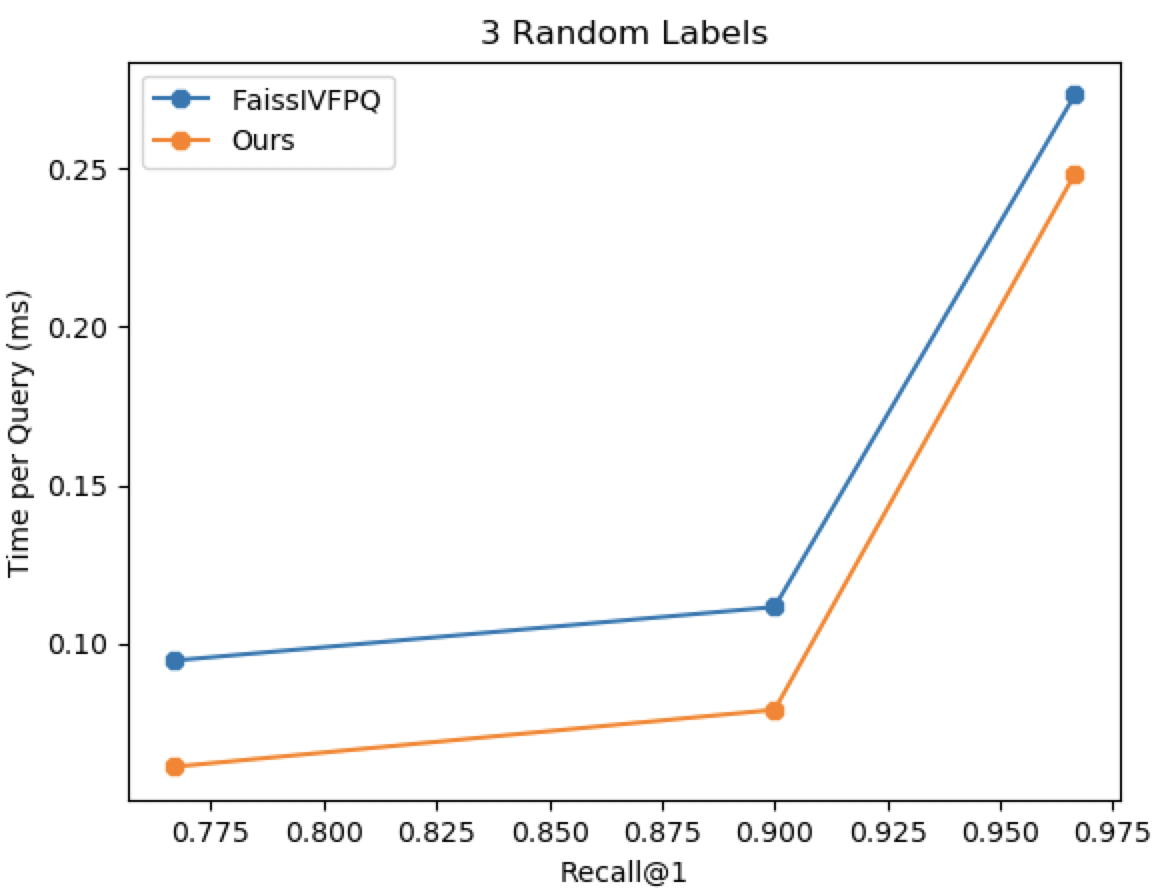
\includegraphics[width=.9\linewidth]{thesis/images/3_random.png}
        % \caption{Results for 3 random label}
        \label{fig:randomexpsub1}
    \end{minipage}%
    \begin{minipage}[b]{.5\textwidth}
        \centering
        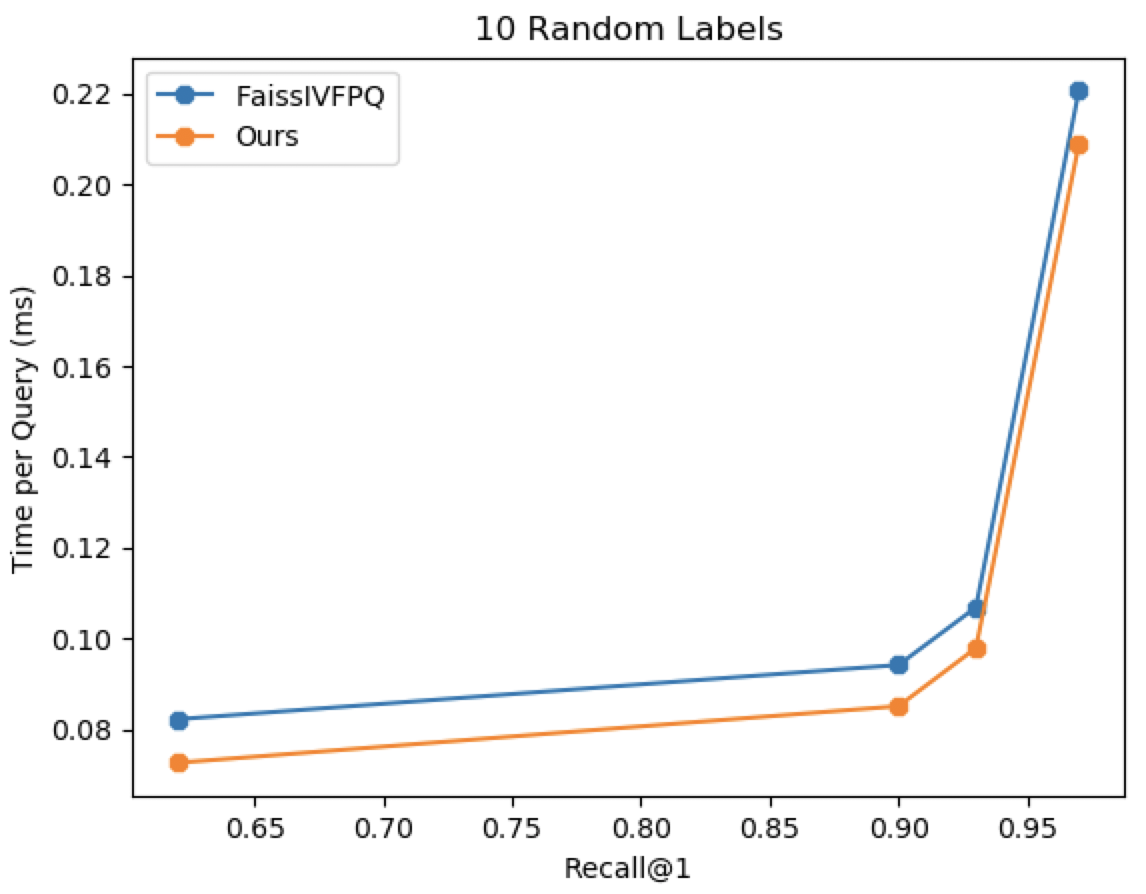
\includegraphics[width=.9\linewidth]{thesis/images/10_random_only_mo1.png}
        % \caption{Results for 10 random label}
        \label{fig:randomexpsub2}
    \end{minipage}
    %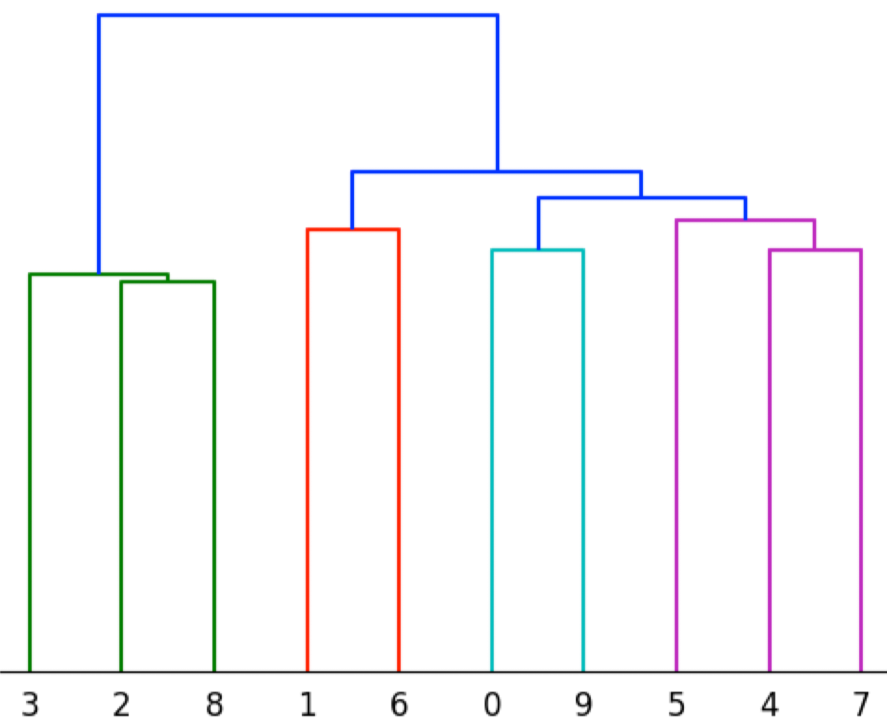
\includegraphics[width=0.40\textwidth]{images/hierfig.png}
    \caption{Comparison of our method with FaissIVFPQ on randomly picked labels as user requirements}
    \label{fig:randomexp}
\end{figure}

According to our scenario, users have wearable devices with a camera, such as wearable glasses or a smart phone. 
When they first start using the image search system, the class recognition system will store the classification labels of the users. 
After storing labels for enough time, we will consider those labels as the user's required class labels.
Then, we select the subspaces, out of all 1140 subspaces, that contain any of those class labels at least $m$ times. 
$m$ is the hyper-parameter to adjust the trade-off between accuracy and speed.
Whenever a new query image comes from the user, we compare the query vector only with the centroids of the selected subspaces to reduce time.
Note that, classification labels are merely a tool for us to categorize the requirements of the users.
Most similar images do not necessarily have the same labels.

In our experiments, two types of tests are conducted. 
The first phase of testing is done with random or hand-picked data to analyze our method thoroughly. 
For the second phase of testing, real data is used to observe whether our method is applicable to real-life scenarios. 
Two phases will be explained in their respective sections.

\subsection*{Experiments with Artificial Data}

Our proposed method is making use of the user requirements to speed up the search for image retrieval. 
In our work, user requirements are represented with the classification labels. 
These are the labels that the users most likely encounter in their daily lives. 
According to our scenario, these labels are extracted with a recognition model included in their device as mentioned earlier in \ref{retrievallabelinfo}. 
In our experiments, we either randomly picked or hand-picked these labels to validate our method with diversified tests.

When the class labels are randomly picked, the results are expected to be the worst for our method. 
The reason is that randomly picked labels would not be related to each other, whereas in real life user-required labels might have similar images. 
Because the task is similarity search, similar images with different labels are closer in the search space, therefore it is easier to reduce the space more.
For example, randomly picked labels might include labels such as volcano, waterfall, ski slope at the same time, whereas user-required labels are more likely to have labels such as campus, library-outdoor, library-indoor.
Having said that, results for randomly picked labels can be seen in the figure \ref{fig:randomexp}.
In both of the figures, it can be clearly seen that our method surpasses the baseline as our method can perform faster with the same accuracy.

Further experiments are done with hand-picked labels. 
In these experiments, labels are picked intuitively considering their relevancy. 
The results can be seen in the figure \ref{fig:handpickedexp}. 
We can see again that our method performs better than the baseline.

When the number of labels chosen for user requirements is relatively small, our method outperforms the baseline method.
However, as the number of labels go up, our method starts to behave similarly to the baseline.
The reason is that we only search the sub-spaces in our search space which contains at least $k$ of any required labels. 
When the number of labels is high, it becomes harder to exclude some sub-spaces. Because almost all of them has at least one of any required labels. 
That is why, our method works if user required labels are relatively small which actually makes sense because if the user requires many labels, they do not need to use our system as they can use generic model for their need.


\begin{figure}
    \centering
    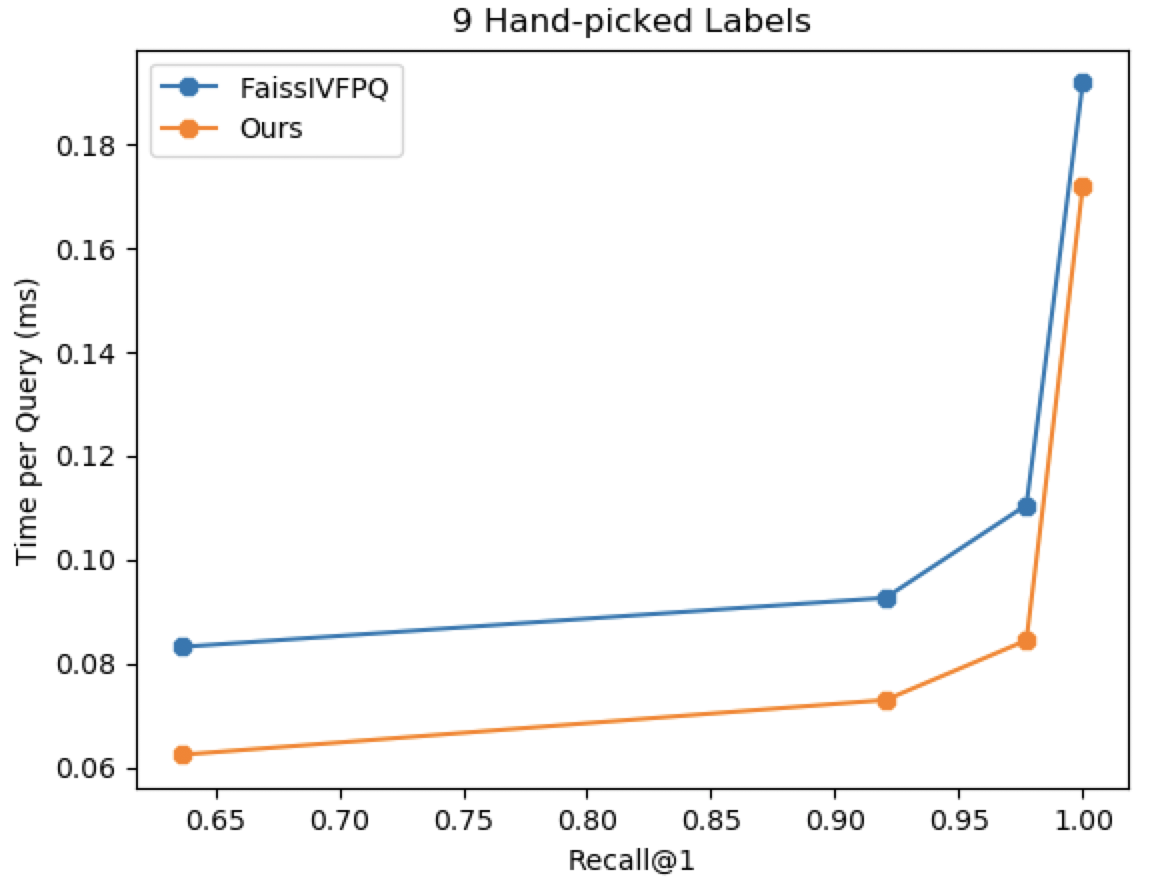
\includegraphics[width=0.8\textwidth]{thesis/images/9_handpicked.png}
    \caption{Comparison of our method with FaissIVFPQ on hand-picked labels as user requirements}
    \label{fig:handpickedexp}
\end{figure}

\subsection*{Experiments with Real Data}

The real data for this phase is obtained using GoPro Hero8 with a chest mount. 
Daily v-logs are taken for 2 days, first day data is used for extracting user required classification labels and second day data is used to actually test our method.

Daily v-logs are recorded for 2 days for nearly a total of 2 hours. 
Videos are mostly taken when the subject is on the move to prevent recording constant same scenes.
For each day, videos are sampled with a ratio of 1 frame per 10 seconds. 
426 frames for the first day and 280 frames for the second day is obtained.

First day frames are classified with a pre-trained ResNet with 18 layers~\cite{resnet}. 
73 different labels are recognized from 426 frames with many misclassified labels such as airplane cabin, airport terminal, berth, catacomb and many more. 
Many labels are predicted only once or with little probabilities. Therefore, a limit is put to probability and minimum occurrence to exclude some of the labels. 
We refer to this method as "Ours-limited".

Second day frames(280) are converted to query vectors with the usual process, explained in \ref{extractdeepfeatures}. The result of searching with these query images is shown in the figure \ref{fig:realdataexp}. 
There are 1140 sub-spaces in the search space. Our method could reduces the area to only 1108 sub-spaces using 73 user-required labels. 
Thus, our method fails to speed up the baseline for the real-life experiment. 
Limited version of our method is obtained by a limit to probability by 50 percent classification accuracy and at least 3 minimum occurrence of labels to count them as requirements.
However, excluding some classified labels reduced the accuracy of "Ours-limited".
Results will be discussed more thoroughly in the next chapter and further experiment results will be shown in \ref{Appen} Additional Results.

\begin{figure}
    \centering
    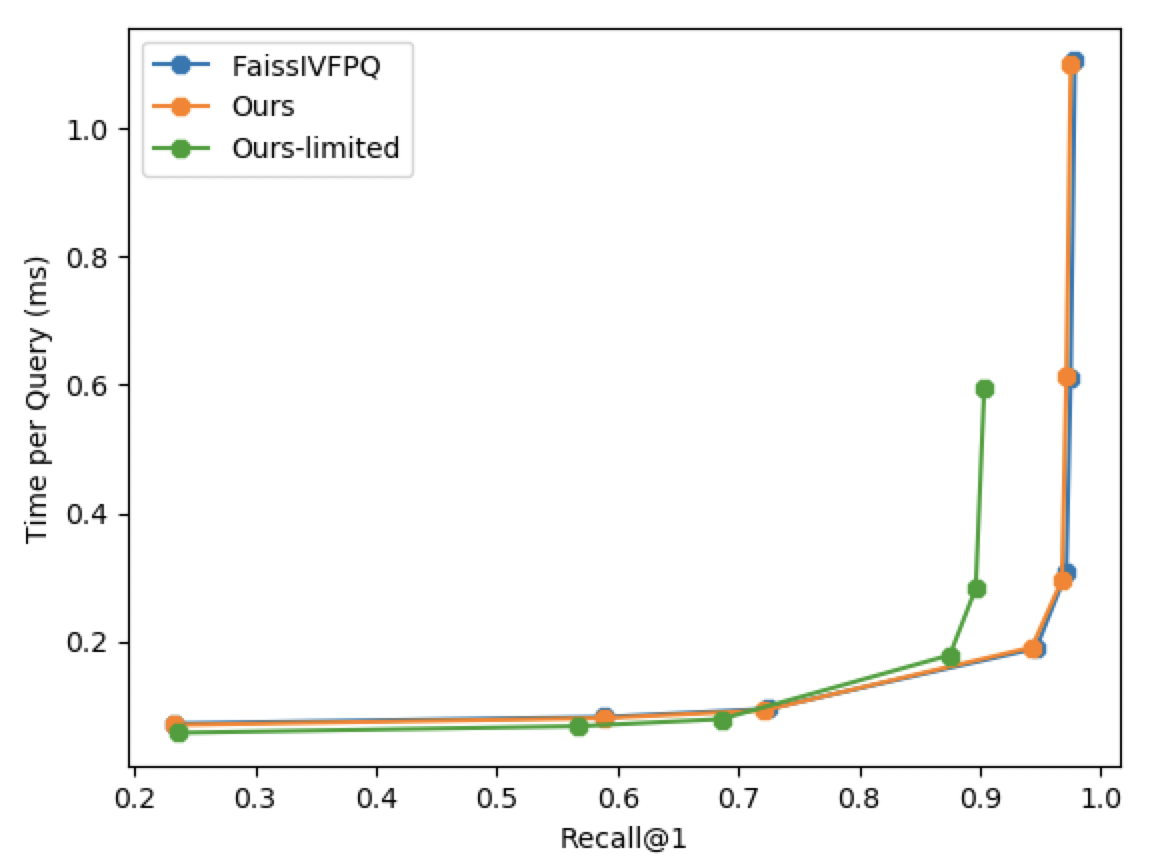
\includegraphics[width=0.8\textwidth]{thesis/images/real_data_experiment.png}
    \caption{Comparison of our method with FaissIVFPQ in a real-life experiment}
    \label{fig:realdataexp}
\end{figure}

